\documentclass[10pt]{beamer}

\usetheme[progressbar=frametitle]{metropolis}
\usepackage{appendixnumberbeamer}

\usepackage{booktabs}
\usepackage[scale=2]{ccicons}

\usepackage{pgfplots}
\usepgfplotslibrary{dateplot}

\usepackage{xspace}
\newcommand{\themename}{\textbf{\textsc{metropolis}}\xspace}

\usepackage[brazilian]{babel}
\usepackage[utf8]{inputenc}
\usepackage[T1]{fontenc}

\title{UNIVERSIDADE DE ITAÚNA}
\subtitle{Aprendizado de Máquina Aplicado à Valoração de Redações}
% \date{\today}
\date{19 de Junho de 2017}
\author{\textbf{Graduando:} Eugênio Cunha \\ \textbf{Orientador:} Dr. Marco Túlio Alves N Rodrigues}
\institute{{Departamento de Ciência da Computação \small} \\ {Bacharelado em Ciência da Computação \small}}
\titlegraphic{\hfill
\includegraphics[height=1.5cm]{images/uit.pdf}}

\begin{document}

\maketitle

\begin{frame}{Aprendizado de Máquina Aplicado à Valoração de Redações}
  \setbeamertemplate{section in toc}[sections numbered]
  \tableofcontents[subsectionstyle=show]
\end{frame}

\section{Introdução}

  \subsection{Problema de Pesquisa}
    \begin{frame}[fragile]{Problema de Pesquisa}
    O decreto 79.298, de 24 de Fevereiro de 1977 definiu a “inclusão obrigatória da prova ou questão de redação em língua portuguesa” nos concursos e vestibulares (Art. 1 o , alínea d).
    \end{frame}

    \begin{frame}[fragile]{Problema de Pesquisa}
    No ENEM cada redação foi avaliada por, pelo menos, dois avaliadores, de forma independente ~\cite{edital_enem:2016}.
    \begin{figure}[H]
    \begin{center}
        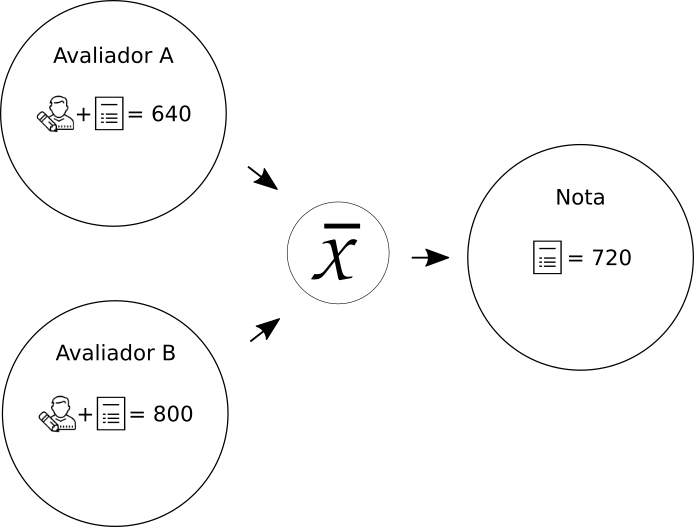
\includegraphics[scale=0.50]{images/correction_redaction_enem.png}
    \end{center}
    \end{figure}
    \end{frame}

    \begin{frame}[fragile]{Problema de Pesquisa}
    Dados da avaliação de redações do ENEM 2016 ~\cite{paq_a:2016}.
    \begin{figure}[H]
    \begin{center}
        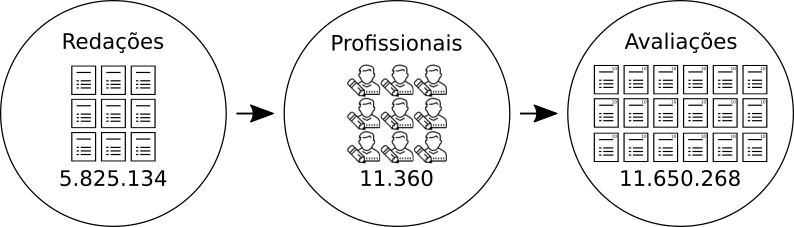
\includegraphics[scale=0.50]{images/enem_2016.png}
    \end{center}
    \end{figure}
    \end{frame}

    \begin{frame}[fragile]{Problema de Pesquisa}
    Dado um corpus de redações, classificar as competências exigidas em um texto de redação.
    \begin{figure}[H]
    \begin{center}
        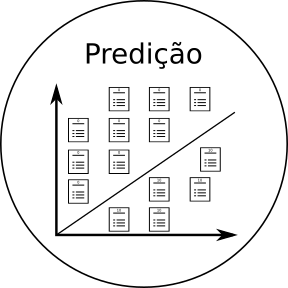
\includegraphics[scale=0.50]{images/prediction.png}
    \end{center}
    \end{figure}
    \end{frame}

  \subsection{Objetivos}
    \begin{frame}[fragile]{Objetivos}
    Induzir um modelo de Aprendizado de Máquina a classificar as competências exigidas em um texto de redação.

    \begin{figure}[H]
    \begin{center}
        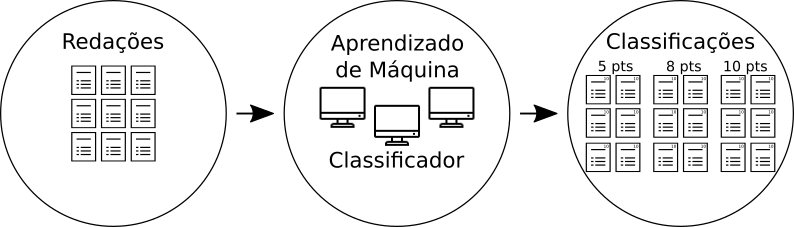
\includegraphics[scale=0.50]{images/automatic_essay_system.png}
    \end{center}
    \end{figure}
    \end{frame}

  \subsection{Motivação}
    \begin{frame}[fragile]{Motivação}
    Aprendizado de Máquina está no centro de muitos avanços tecnológicos, alcançado áreas antes exclusivas de seres humanos.
    \begin{figure}[H]
    \begin{center}
        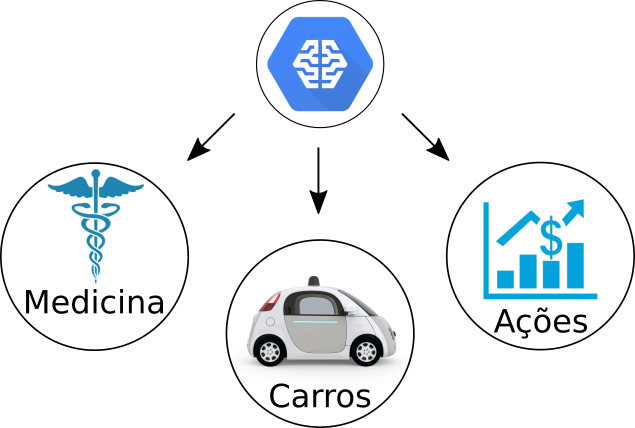
\includegraphics[scale=0.50]{images/machine_learn.png}
    \end{center}
    \end{figure}
    \end{frame}

\section{Trabalhos Relacionados}
  \begin{frame}[fragile]{Matriz de Competências}
  Silva, Carvalho ~\cite{silvio_taynan:2017} cita em seu estudo que à prova de redação do ENEM é avaliada levando em conta uma matriz de referência elaborada pelo INEP.

\begin{table}[H]
\centering
\begin{tabular}{|l|l|l|}
\hline
\textbf{I} & {Demonstrar domínio da norma padrão da língua escrita.}\small & 200 \\ \hline
\textbf{II} & \begin{tabular}[c]{@{}l@{}}Compreender a proposta de redação e aplicar conceitosdas \\ varias áreas de conhecimento para desenvolver o tema, dentro \\ dos limites estruturais do textodissertativo-argumentativo em \\ prosa.\end{tabular} & 200 \\ \hline
\textbf{III} & \begin{tabular}[c]{@{}l@{}}Selecionar, relacionar, organizar e interpretar informações, \\ fatos, opiniões e argumentos em defesa de um ponto de vista.\end{tabular} & 200 \\ \hline
\textbf{IV} & \begin{tabular}[c]{@{}l@{}}Demonstrar conhecimento dos mecanismos linguísticos \\ necessários para a construção da argumentação.\end{tabular} & 200 \\ \hline
\textbf{V} & \begin{tabular}[c]{@{}l@{}}Elaborar proposta de intervenção para o problema abordado, \\ respeitando os direitos humanos.\end{tabular} & 200 \\ \hline
\end{tabular}
\end{table}


  \end{frame}

  \begin{frame}[fragile]{Aprendizado de Máquina}
  \end{frame}

  \begin{frame}[fragile]{Orange Data Mining}
  \end{frame}

\section{Metodologia}
  \begin{frame}[fragile]{Coleta de Dados}
  \end{frame}

  \begin{frame}[fragile]{Orange Data Mining}
  \end{frame}
  
  \begin{frame}[fragile]{Métricas de Desempenho}
  \end{frame}

\section{Resultados Preliminares}
  \begin{frame}[fragile]{Adversidades}
  \end{frame}

  \begin{frame}[fragile]{Resultado da Avaliação}
  \end{frame}

  \begin{frame}[fragile]{Curva ROC}
  \end{frame}

  \begin{frame}[fragile]{Matriz de Confusão}
  \end{frame}

\section{Plano de Trabalho}
  \begin{frame}[fragile]{Plano de Atividades}
  \end{frame}

% \appendix desliga o slide da barra de progresso
\appendix
\begin{frame}[allowframebreaks]{References}

  \bibliography{bib}
  \bibliographystyle{abbrv}
\end{frame}

\end{document}